\documentclass[12pt]{beamer}
% \usetheme{umbc4}
\usetheme{moloch}

\usepackage{amsmath,amscd}
\usepackage{fontspec}
\usepackage{unicode-math}
\usepackage{pifont}
\usepackage{xcolor}
\usepackage[dvipsnames]{xcolor}
\usepackage{listings}
\usepackage{minted}
\usepackage{tikz}
\usepackage{twemojis}
\usepackage{nicematrix}

\usetikzlibrary{fit}

\setmonofont{DejaVu Sans Mono}

% Set the title bar to black background with white text
\setbeamercolor{frametitle}{bg=black, fg=white}

% Ensure other structural elements (bullets, etc.) are visible
\setbeamercolor{structure}{fg=white}

\setmainfont{Libertinus Serif}
\setsansfont{Libertinus Sans}
\setmathfont{STIX Two Math}

% Define colors for syntax highlighting
\definecolor{codegreen}{rgb}{0,0.6,0}
\definecolor{codegray}{rgb}{0.5,0.5,0.5}
\definecolor{codecoffee}{rgb}{0.75,0.6,0.3}
\definecolor{question}{rgb}{1.0,0.75,0.1}
\definecolor{lightblue}{rgb}{0.55,0.75,0.9}
\definecolor{yellow}{rgb}{1.0, 1.0, 0.0}
\definecolor{codecomment}{rgb}{0.97, 0.74, 0.4}
\definecolor{codepy}{rgb}{0.9, 0.85, 0.85} %{#F8BC65}
\definecolor{funcColor}{rgb}{0.47, 0.6, 0.8}
\definecolor{midgray}{rgb}{0.4, 0.4, 0.3}
\definecolor{indexwhite}{rgb}{0.9, 0.9, 0.9}

\setbeamercolor{background canvas}{bg=black}
\setbeamercolor{normal text}{fg=white}


\newcommand{\FrameTitle}[2]{\frametitle{#1 \hfill \small\textnormal{\textcolor{midgray}{#2}}}}
\newcommand{\snl}{\vspace*{8pt}\\}
\newcommand{\nl}{\vspace*{1em}\\}
\newcommand{\vsp}{\vspace*{1em}}
\newcommand{\smallvspace}{\vspace*{0.5em}}

\newcommand{\Matrix}[1]{\textbf{#1}}
\newcommand{\Vector}[1]{\textbf{#1}}
\newcommand{\Scalar}[1]{\textnormal{#1}}
\newcommand{\Quiz}[1]{{\Large\textbf{\color{question}{#1}}}}

\begin{document}
\title{\center{Applied Linear Algebra \\\vsp Finite-Dimensional Vector Spaces \\}}

\author{\center{Devi Prasad M \\ Manipal School of Information Sciences \\ Manipal \\}}
\date{\center{August 2026}}
\maketitle


\begin{frame}\FrameTitle{Scalars}{Unit 1}
    \begin{itemize}
        \item A scalar is a single value, which can be an integer, a real number, or a complex number.
        \item Scalars are the simplest mathematical objects.
    \end{itemize}
    \vsp
    {\Quiz{Quiz}}\snl
    {\color{white}{\large{Name a few good examples of scalars.}}}
\end{frame}

\begin{frame}\FrameTitle{Vectors}{Unit 1}
    \begin{itemize}
        \item A vector is a more structured mathematical object.
        \item A vector is an ordered sequence of scalars.\snl
        \item[] \Vector{v} $ = (a_1, a_2, \ldots, a_n) \in \mathbb{R}^n$
        \item[] \hspace*{1em} $where \ \mathbb{R}^n$ is the set of all n-dimensional real vectors. \snl
        \item[]$\Vector{v} = (0.35, 0.71, 0.23, 0.8) \in \mathbb{R}^4$ \snl
        \item[]$\Vector{v} = (0.35) \in \mathbb{R}^{\textbf{\color{yellow}{?}}}$ \snl
        \item[]$\Vector{v} = (0.35, 0.71) \in \mathbb{R}^{\textbf{\color{yellow}{?}}}$ \snl
        \item[]$\Vector{v} = () \in \mathbb{R}^{\textbf{\color{yellow}{?}}}$ \snl
    \end{itemize}
\end{frame}

\begin{frame}\FrameTitle{Vectors}{Unit 1}
    Let \Matrix{A} be a $m \times n$ matrix.\snl
    The $n$ columns of \Matrix{A} are vectors in $\mathbb{R}^m$.\snl

    \textbf{Example}: A matrix with 4 column vectors in $\mathbb{R}^5$
    \[
    \begin{bNiceMatrix}[
        margin=2pt,
        code-after = {
            \tikz[remember picture, overlay]
            \node [
                draw=yellow,            % yellow border line
                %fill=blue!10,          % Very light blue interior fill
                %opacity=0.9,           % High transparency for the shape
                text opacity=1,         % Keeps numbers dark and 100% readable
                thick,                  % outline border style
                %rounded corners=5pt,   % Smooths the rectangle corners perfectly
                inner xsep=4pt,        % Padding to prevent numbers from touching the border
                inner ysep=6pt,        % Vertical padding at the top and bottom
                fit = (1-2) (5-2)      % Fits from Row 1, Col 2 down to Row 5, Col 2
            ] {} ;
        }
    ]
    .1 & .2 & .3 & 0.6\\
    .4 & .5 & .6 & 0.12\\
    .7 & .8 & .9 & 0.18\\
    .11 & .12 & .13 & 0.26\\
    .21 & .22 & .23 & 0.33\\
    \end{bNiceMatrix}
    \]
\end{frame}

\begin{frame}\FrameTitle{Vectors}{Unit 1}
    A vector can be represented as a row or column of scalars.\\
    \begin{columns}[T]
        \begin{column}{0.48\textwidth}
            \centering{\color{lightblue}{Row vector}}
            \[
            \begin{pmatrix}
                0.35, & 0.71, & 0.23, & 0.8
            \end{pmatrix}
            \]
        \end{column}
        \vline{\color{darkgray}\vrule width 0.2pt}
        \begin{column}{0.48\textwidth}
            \centering{\color{lightblue}{Column vector}}
            \[
            \begin{bmatrix}
                0.35 \\ 0.71 \\ 0.23 \\ 0.8
            \end{bmatrix}
            \]
        \end{column}
    \end{columns}
\end{frame}

\begin{frame}\FrameTitle{Unit Vector}{Unit 1}
    A \emph{unit vector} is a vector with all elements equal to zero,
    except one element which is equal to one.
    \vsp

    The \emph{i}-th unit vector (of size \emph{n}) is the unit vector
    with \emph{i}-th element one, and denoted $\Vector{e}_i$.

    \[
        \Vector{e}_1 = \begin{bmatrix}
            1 \\ 0 \\ 0 \\ \vdots \\ 0
        \end{bmatrix}, \quad
        \Vector{e}_2 = \begin{bmatrix}
            0 \\ 1 \\ 0 \\ \vdots \\ 0
        \end{bmatrix}, \quad
        \Vector{e}_3 = \begin{bmatrix}
            0 \\ 0 \\ 1 \\ \vdots \\ 0
        \end{bmatrix}
    \]
\end{frame}

\begin{frame}\FrameTitle{Unit Vector}{Unit 1}
    The \emph{i}-th unit vector (of size \emph{n}) is the unit vector
    with \emph{i}-th element one, and denoted $\Vector{e}_i$.

    \begin{equation}
        (\Vector{e}_i)_j = \begin{cases}
            \ 1 & i = j \\
            \ 0 & otherwise
        \end{cases}
    \end{equation}
    for $i,j = 1, \ldots, n$.

    \vsp
    $\Vector{e}_i$ is an \emph{n}-vector. $(\Vector{e}_i)_j$ is a number, its \emph{j}-th entry.
\end{frame}

\begin{frame}\FrameTitle{Ones Vector}{Unit 1}
    A \emph{ones vector} is a vector with all elements equal to one.
    \vsp
    The \emph{n}-dimensional ones vector is denoted $\Vector{1}_n$.

    \[
        \Vector{1}_3 = \begin{bmatrix}
            1 \\ 1 \\ 1
        \end{bmatrix}, \quad
        \Vector{1}_4 = \begin{bmatrix}
            1 \\ 1 \\ 1 \\ 1
        \end{bmatrix}, \quad
        \Vector{1}_5 = \begin{bmatrix}
            1 \\ 1 \\ 1 \\ 1 \\ 1
        \end{bmatrix}
    \]
\end{frame}

\begin{frame}\FrameTitle{Properties of Vector Addition}{Unit 1}
    For any $n$-vectors \Vector{a}, \Vector{b}, and \Vector{c}, the following properties hold:
    \begin{itemize}
        \item Vector addition is \emph{commutative}: \Vector{a} + \Vector{b} = \Vector{b} + \Vector{a}.
        \item Vector addition is \emph{associative}: (\Vector{a} + \Vector{b}) + \Vector{c} = \Vector{a} + (\Vector{b} + \Vector{c}). We can therefore
        write both as \Vector{a} + \Vector{b} + \Vector{c}.
        \item \Vector{a} + \textbf{0} = \Vector{0} + \Vector{a} = \Vector{a}. Adding the zero vector to a vector has no effect.$^{\dagger}$
        \item \Vector{a} - \Vector{a} = \Vector{0}. Subtracting a vector from itself gives the zero vector.
    \end{itemize}
    \vsp
    {\color{question}{Can you think of the geometric interpretation of these properties?}}
    \vfill
    $^{\dagger}$ The size of the zero vector follows from the context
\end{frame}

\begin{frame}\FrameTitle{Vector Addition}{Unit 1}
    \begin{columns}[c]
        \begin{column}{0.8\textwidth}
            \begin{center}
            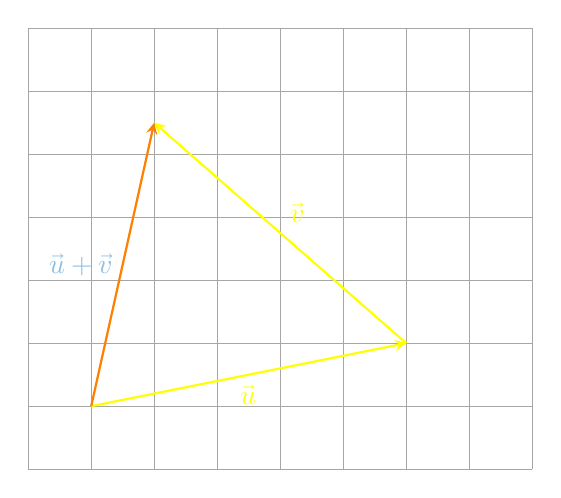
\begin{tikzpicture}[scale=0.8]
                % 1. Draw the square grid
                \draw[thin, gray!70] (0,0) grid (8,7);

                \draw[thick, -stealth, yellow] (1,1) -- (6,2)
                    node[midway, below, yellow] {$\vec{u}$};
                \draw[thick, -stealth, yellow] (6,2) -- (2,5.5)
                    node[midway, above right, yellow] {$\vec{v}$};

                \draw[thick, -stealth, orange] (1,1) -- (2,5.5)
                    node[midway, left, lightblue] {$\vec{u} + \vec{v}$};
            \end{tikzpicture}
            \end{center}
        \end{column}
    \end{columns}
\end{frame}


\begin{frame}\FrameTitle{Scalar-vector multiplication}{Unit 1}
    For any $\Vector{a} \in \mathbb{R}^n$, and scalars $\alpha, \beta, \gamma \in \mathbb{R}$,
    the following properties hold:
    \begin{itemize}
        \item scalar-vector multiplication is \emph{commutative}: $\alpha \Vector{a} = \Vector{a} \alpha$.
        \item scalar-vector multiplication is \emph{associative}: $(\beta \gamma) \Vector{a} = \beta (\gamma \Vector{a})$.
        \item $\Scalar{1} \Vector{a} = \Vector{a}$. Multiplying a vector by the scalar 1 has no effect.
        \item $\Scalar{0} \Vector{a} = \Vector{0}$. Multiplying a vector by the scalar 0 gives the zero vector.
        \item $\beta (\Vector{a} + \Vector{b}) = \beta \Vector{a} + \beta \Vector{b}$. Scalar multiplication distributes over vector addition.
        \item $(\beta + \gamma) \Vector{a} = \beta \Vector{a} + \gamma \Vector{a}$. The distributive property of scalar-vector multiplication.

    \end{itemize}
\end{frame}

\begin{frame}\FrameTitle{Vector Spaces}{Unit 1}
A vector space $V$ is a set endowed with a rule for addition and a
rule for scalar multiplication
    \begin{align*}
        +: V \times V \rightarrow V \\
        \cdot: \mathbb{R} \times V \rightarrow V
    \end{align*}

such that the following axioms hold for all $\Vector{u}, \Vector{v}, \Vector{w} \in V$ and all scalars $c_{1}, c_{2} \in \mathbb{R}$:
    \begin{enumerate}
        \item $\Vector{u} + \Vector{v} = \Vector{v} + \Vector{u}$
        \item $(\Vector{u} + \Vector{v}) + \Vector{w} = \Vector{u} + (\Vector{v} + \Vector{w})$
        \item $\Vector{v} + \Vector{0} = \Vector{v}$
        \item $\Vector{v} + (-\Vector{v}) = \mathbf{0}$ where $-\Vector{v}$ is the unique additive inverse of $\Vector{v}$
        \item $c_1 \cdot (\Vector{v} + \Vector{w}) = c_1 \cdot \Vector{v} + c_1 \cdot \Vector{w}$
        \item $(c_1 + c_2) \cdot \Vector{v} = c_1 \cdot \Vector{v} + c_2\cdot \Vector{v}$
        \item $c_1 \cdot (c_2 \cdot \Vector{v}) = (c_1 c_2) \cdot \Vector{v}$
        \item $\Scalar{1} \cdot \Vector{v} = \Vector{v}$
    \end{enumerate}
\end{frame}

\begin{frame}\FrameTitle{Vector Spaces}{Unit 1}
    {\center{\Large\textbf{Examples of Vector Spaces}}}
\end{frame}

\begin{frame}\FrameTitle{Vector Spaces - Questions}{Unit 1}
    \vsp
    \begin{enumerate}
        \item {\color{question}{\large{is a $3 \times 2$ matrix of $\mathbb{R}$ a vector space?}}}
        \item {\color{question}{\large{is a $3 \times 2$ matrix of $\mathbb{R}$ with non-negative entries a vector space?}}}
        \item {\color{question}{\large{is a $m \times n$ matrix of $\mathbb{R}$ a vector space?}}}
    \end{enumerate}
\end{frame}

\begin{frame}\FrameTitle{Vector Spaces - Questions}{Unit 1}
    \vsp
    \begin{enumerate}
    \item {\textcolor{question}{
        Suppose addition in $\mathbb{R}^2$ adds an extra 1 to each component.
        With scalar multiplication unchanged, which rules are broken?
    }}
    \nl
    \item {\textcolor{question}{
        Show that the set of all positive real numbers, with $x + y$ and $cx$ redefined to
        equal the usual $xy$ and $x^c$, is a vector space. What is the ``zero vector''?
    }}
    \end{enumerate}
\end{frame}


\begin{frame}\FrameTitle{Linear Combinations}{Unit 1}
    if $\Vector{a}_1, \ldots, \Vector{a}_m$ are \emph{n}-vectors, and $\beta_1,\ldots,\beta_m$ are scalars,
    the \emph{n}-vector

    \[
        \beta_1 \Vector{a}_1 + \cdots + \beta_m \Vector{a}_m
    \]
    is called the \emph{linear combination} of the vectors $\Vector{a}_1,\ldots,\Vector{a}_m$.

    \vsp

    The scalars $\beta_1,\ldots,\beta_m$ are called the \emph{coefficients}
    of the linear combination.
\end{frame}

\begin{frame}\FrameTitle{Linear combination of unit vectors}{Unit 1}
    \[
        \begin{bmatrix}
            8.3 \\
            -0.2 \\
            10
        \end{bmatrix} =
        8.3 \begin{bmatrix}
            1 \\
            0 \\
            0
        \end{bmatrix} +
        (-0.2)\begin{bmatrix}
            0 \\
            1 \\
            0
        \end{bmatrix} +
        10\begin{bmatrix}
            0 \\
            0 \\
            1
        \end{bmatrix}
    \]
\end{frame}


\begin{frame}\FrameTitle{Affine Combination}{Unit 1}
    When the coefficients sum to one, i.e., $\beta_1 + \cdots + \beta_m = 1$,
    the linear combination is called an \emph{affine combination}.

    \vsp

    When the coefficients in an affine combination are nonnegative,
    it is called a \emph{convex combination}, or a \emph{weighted average}.
\end{frame}

\begin{frame}\FrameTitle{Inner Product}{Unit 1}
    \begin{definition}[Inner or Dot Product]
        The inner product of two $n$-vectors is defined as the \emph{scalar}
        \[
            \Vector{a}^{\textrm{T}}\,\Vector{b} = a_1b_1 + a_2b_2 + \ldots + a_nb_n,
        \]
        the sum of the products of corresponding entries.
    \end{definition}
    \vsp
    If $\Vector{a}$, $\Vector{b}$, and $\Vector{c}$ are vectors of the same size, and {\color{yellow}$\gamma$} is a scalar, then the following hold:\vspace*{2pt}\\
    \begin{enumerate}
        \item \emph{Commutativity}: $\Vector{a}^{\textrm{T}}\,\Vector{b} = \Vector{b}^{\textrm{T}}\,\Vector{a}$ aka \emph{symmetric}\vspace*{3pt}\\
        \item \emph{Associativity with scalar multiplication}: $(\gamma \Vector{a})^{\textrm{T}}\,\Vector{b} = \gamma (\Vector{a}^{\textrm{T}}\,\Vector{b})$ \vspace*{3pt}\\
        \item \emph{Distributivity with vector addition}: $(\Vector{a}+\Vector{b})^{\textrm{T}}\,\Vector{c} = \Vector{a}^{\textrm{T}}\,\Vector{c} + \Vector{b}^{\textrm{T}}\,\Vector{c}$
    \end{enumerate}
\end{frame}

\begin{frame}\FrameTitle{Inner Product: Special Examples}{Unit 1}
    \begin{itemize}
        \item \emph{Unit vector}. $e^{\textrm{T}}_i \Vector{a} = a_i$
        \item \emph{Sum}. $1^{\textrm{T}} \Vector{a}= a_1 + \cdots + a_n$
        \item \emph{Sum of squares}. $\Vector{a}^{\textrm{T}} \Vector{a} = a^2_1 + \cdots + a^2_n$
    \end{itemize}
\end{frame}

\begin{frame}\FrameTitle{Inner Product: Applications}{Unit 1}
    \begin{itemize}
        \item \emph{Co-occurrence}. $\Vector{a}^{\textrm{T}} \Vector{b} = a_1b_1 + \cdots + a_nb_n$ counts the number of times the two vectors have non-zero entries in the same position.
        \smallvspace
        \item \emph{Weighs, features, and scores}. $\Vector{w}^{\textrm{T}} \Vector{x} = w_1x_1 + \cdots + w_nx_n$
        \smallvspace
        \item \emph{Polynomial evaluation}. $p(x) = a_0 + a_1x + \cdots + a_nx^n = [1, x, \ldots, x^n]^{\textrm{T}}[a_0, a_1, \ldots, a_n]$
        \smallvspace
        \item \emph{Probability and expected values.} $E[X] = \sum_{i=1}^{n} x_i p_i = [x_1, \ldots, x_n]^{\textrm{T}}[p_1, \ldots, p_n]$
    \end{itemize}
\end{frame}


\begin{frame}\FrameTitle{Outer Product}{}
    \begin{definition}[Outer Product]
        The outer product of a \emph{m}-vector \Vector{a} and an \emph{n}-vector \Vector{b} is
        given by $\Vector{a}\Vector{b}^{\textrm{T}}$, which is an m×n matrix
        \[
            \Vector{a}\Vector{b}^{\textrm{T}} = \begin{bmatrix}
                a_1b_1 & a_1b_2 & \cdots & a_1b_n \\
                a_2b_1 & a_2b_2 & \cdots & a_2b_n \\
                \vdots & \vdots & \ddots & \vdots \\
                a_mb_1 & a_mb_2 & \cdots & a_mb_n
            \end{bmatrix},
        \]
        whose entries are all products of the entries of \emph{a} and the entries of \emph{b}.
    \end{definition}

    \vsp
    In general, $\Vector{a}^{\textrm{T}}\,\Vector{b} \neq \Vector{b}^{\textrm{T}}\,\Vector{a}$, \emph{i.e.},
    it is not \emph{symmetric}\vspace*{3pt}\\
\end{frame}



\begin{frame}\FrameTitle{The Zero-Dimensional Vector Space $\mathbb{R}^0$}{Unit 1}
    % 1. Definition Block
    \begin{definition}[The Trivial Space]
        The space $\mathbb{R}^0$ is the unique zero-dimensional real vector space.
        It contains exactly one element, the empty vector $\Vector{v}$:
        \[
            \Vector{v} \in \mathbb{R}^0 \quad \text{where} \quad \Vector{v} = [ ]
        \]
    \end{definition}
\end{frame}

\begin{frame}\FrameTitle{Subspaces}{Unit 1}
    \begin{definition}
        A subspace $W$ of a vector space $V$ is a non-empty subset of $V$
        that is itself a vector space under the same operations of addition
        and scalar multiplication defined on $V$.
    \end{definition}
    \begin{enumerate}
        \item The zero vector of $V$ is in $W$.
        \item If $u, v \in W$, then $u + v \in W$ (closed under addition).
        \item If $c$ is a scalar and $v \in W$, then $cv \in W$ (closed under scalar multiplication).
    \end{enumerate}
\end{frame}

\begin{frame}\FrameTitle{Vector subspaces}{Unit 1}
    Consider all vectors in $\mathbb{R}^2$ whose components are positive or zero. \snl
    This subset is the first quadrant of the x-y plane.\snl
    It is not a subspace of $\mathbb{R}^2$ because it is not closed under scalar multiplication.\snl
    For example, if
    $$
        \Vector{v} = [1, 1]
    $$
    is in the first quadrant,
    then
    $$
        -1 \cdot \Vector{v} = [-1, -1]
    $$
    is not in the first quadrant.
\end{frame}

\begin{frame}\FrameTitle{Subspaces}{Unit 1}
    If we include the third quadrant along with the first, scalar multiplication is closed,
    but the set is still not a subspace because it is not closed under addition. \snl

    For example, if
    $$
        \Vector{u} = [1, 2] \quad \text{and} \quad \Vector{v} = [-2, -1]
    $$
    are in the first and third quadrants, then
    $$
        \Vector{u} + \Vector{v} = [-1, 1]
    $$
    is not in the first or third quadrant.
\end{frame}

\begin{frame}\FrameTitle{Subspaces}{Unit 1}
    The smallest subspace of $\mathbb{R}^2$ that contains
    the first quadrant is the entire space $\mathbb{R}^2$.
\end{frame}

\begin{frame}\FrameTitle{\color{question}{Math vs. Code}}{\twemoji{light bulb}}
    --- Textbooks use \emph{column vectors} for single samples.\snl
    --- {\color{midgray}{PyTorch uses \emph{row vectors} to handle batches.}}\snl

    \begin{itemize}
        \item Single sample $\Vector{x}$ is a column vector.
        \item Forward pass formula:
            \[
            \Vector{y} = \Vector{W}\Vector{x} + \Vector{b}
            \]
            \item Dimensions:
            \[
            \begin{matrix}
            \Vector{y} & = & \Vector{W} & \Vector{x} & + & \Vector{b} \\
            {\color{yellow}{\scriptstyle(c \times 1)}} & & {\color{yellow}{\scriptstyle(c \times d)}} & {\color{yellow}{\scriptstyle(d \times 1)}} & & {\color{yellow}{\scriptstyle(c \times 1)}}
            \end{matrix}
            \]
    \end{itemize}
\end{frame}

\begin{frame}\FrameTitle{\color{question}{Math vs. Code}}{\twemoji{light bulb}}
    --- {\color{midgray}{Textbooks use \emph{column vectors} for single samples.}}\snl
    --- PyTorch uses \emph{row vectors} to handle batches.\snl
    \begin{itemize}
        \item Batch $\Vector{X}$ stacks samples as rows.
        \item PyTorch \emph{nn.Linear} formula:
        \[
        \Vector{Y} = \Vector{X}\Vector{W}^T + \Vector{B}
        \]
        \item Dimensions ($N$ = batch size):
        \[
        \begin{matrix}
        \Vector{Y} & = & \Vector{X} & \Vector{W}^T & + & \Vector{B} \\
        {\color{yellow}{\scriptstyle(N \times c)}} & & {\color{yellow}{\scriptstyle(N \times d)}} & {\color{yellow}{\scriptstyle(d \times c)}} & & {\color{yellow}{\scriptstyle(1 \times c)}}
        \end{matrix}
        \]
    \end{itemize}
\end{frame}

\begin{frame}\FrameTitle{\color{question}{NumPy and PyTorch}}{\twemoji{light bulb}}
    The standard convention for data analysis and machine learning is that
    \begin{itemize}
        \item[---] rows represent samples or observations: \textcolor{brown}{\textbf{axis 0}}
        \item[---] columns represent features or attributes: \textcolor{brown}{\textbf{axis 1}}
    \end{itemize}
\end{frame}

\end{document}